\section{Cenários Financieros}



\section{Introdução e Contexto}

O Programa de Pleno Pagamento das Dívidas dos Estados – PROPAG, instituído por meio da Lei Complementar n º 212 de 13 de janeiro de 2025, foi concebido como uma forma estratégica de oportunizar a recuperação e o equilíbrio fiscal dos estados, com a possibilidade da revisão dos termos das dívidas que estes possuem com a União, priorizando investimentos em áreas prioritárias, de grande interesse social.

No âmbito do Propag, por meio do Decreto nº 12.433 de 14 de abril de 2025, foi instituído do programa Juros por Educação, que tem como objetivo principal, priorizar investimentos em educação profissional de tecnológica de nível médio (EPTNM).

Este programa determina que, no mínimo, 60\% (sessenta por cento) dos recursos provenientes dos juros não pagos à união e dos oriundos do Fundo de Equalização Federativa (FEF), sejam investidos em iniciativas que promovam a expansão, a manutenção e o fortalecimento da educação profissional e tecnológica em nível médio nos estados, objetivando alcançar as metas de anuais de desempenho estabelecidas pelo Plano Nacional de Educação (PNE).

Pensando também em atender aos estados que estão em dia com suas responsabilidades fiscais e que não possuem dívidas com a União, o programa permite que estes estados também possam aderir ao programa e possam participar da distribuição dos recursos que serão aportados Fundo de Equalização Federativa.

Para oportunizar a participação dos estados que não possuem dívidas com a União e, de certa forma, beneficiar estes estados, será criado o Fundo de Equalização Federativa (FEF), onde os estados endividados que optarem por aderir ao Propag, deverão aportar anualmente um percentual do seu saldo devedor para compor esse fundo, o qual será distribuído anualmente entre todos os estados que aderirem ao Propag na proporção determinada pelo art. 46, incisos I e II do Decreto 12.433/2025.

Quanto aos prazos, os estados têm até o dia 31 de dezembro de 2025 para aderirem ao Propag, devendo para tanto, formalizar sua intenção por meio do envio de um ofício do Chefe do Poder Executivo do estado à Secretaria do Tesouro Nacional, indicando sua intenção de aderir ao Propag, a indicação dos ativos que pretende oferecer à União e a indicação de lei autorizativa devidamente publicada no Diário Oficial.

Os estados deverão apresentar Plano de Aplicação dos Recursos, um para o exercício de 2025 e outro para o exercício de 2026, contemplando, no mínimo, a previsão total de matrículas para o ano subsequente, indicativo do quantitativo de matrículas a serem realizadas pela rede estadual e por meio de parcerias, a previsão de cursos e matrículas e suas justificativas de escolha e a estimativa de investimentos complementares para cumprir o mínimo de 60\% (sessenta por cento) em educação profissional e tecnológica de nível médio.

O prazo para apresentar os Planos de Aplicação para 2025 e 2026 é de até 30 dias após a assinatura do Termo de Aditivo pelo estado, ou até 30 de outubro de 2025, o que ocorrer primeiro. Após 30 de outubro de 2025, os estados deverão apresentar o Plano de Aplicação no momento da assinatura do Termo Aditivo. 

Os demais 40\% (quarenta por cento) dos recursos oriundos do Propag, poderão ser investidos em universidades estaduais, infraestrutura educacional, saneamento, habitação, segurança pública e adaptação climática.

Para 2025, as metas a serem alcançadas seguem os parâmetros do PNE vigente (2014 – 2025). Para 2026, caso seja aprovado o novo PNE, as metas deverão ser alteradas para obedecer aos parâmetros deste novo plano.


\section{Projeção das dívidas}

Conforme relatado, a criação do Programa de Pleno Pagamento das Dívidas dos Estados, o PROPAG, tem como objetivo principal, proporcionar aos estados que possuem dívidas com a União, condições de refinanciar e quitar suas dívidas no prazo de 360 meses, com a possibilidade de zerar os juros incidentes sobre o saldo devedor, permitindo o equilíbrio financeiro destes entes, culminando na retomada do crescimento e do desenvolvimento econômico e social.

Com o objetivo de demonstrar as possíveis vantagens financeiras que a adesão ao Propag poderá trazer aos estados, buscou-se apresentar uma simulação da evolução do crescimento das dívidas de alguns estados nos últimos 5 anos (2021 – 2025), bem como, uma simulação da projeção destas dívidas nos próximos 10 anos (2026 – 2035), a qual foi representada em um quadro evolutivo, simulando 3 cenários diferentes, onde estes estados, supostamente, optam primeiro, por não aderir ao programa Propag, num segundo cenário, aderindo e fazendo um abatimento do saldo devedor de 20\% (vinte por cento) e, num  terceiro cenário, optando por aderir sem fazer nenhum abatimento no saldo devedor. 

Seguindo a tabela evolutiva, apresentamos um gráfico comparativo, demonstrando a evolução do saldo devedor em cenários simulados.

Cabe lembrar que, por se tratar de um refinanciamento das dívidas estaduais feitas com base na tabela Price, com correção pelo índice IPCA, pelo prazo de 360 meses, a tendência de redução nos valores das prestações, começa a ser perceptível a partir da metade final do prazo, entre os últimos anos. 


\begin{figure}[htbp!]
	\centering
	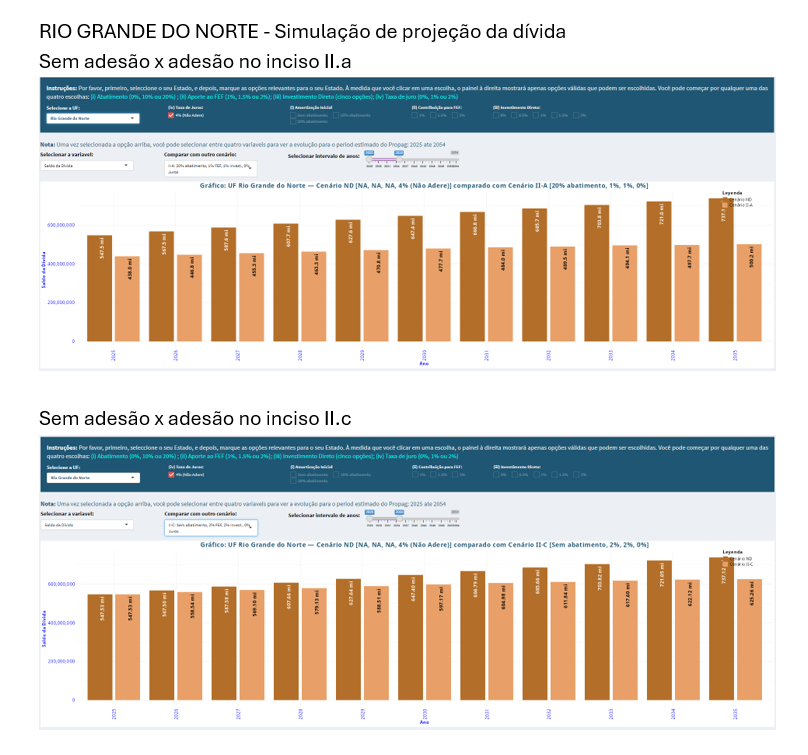
\includegraphics[width=1\textwidth]{images/7a.png}
	\caption{Aba E: Análise de Cenários EPT} 
	\label{fig:7a}
\end{figure}


\begin{figure}[htbp!]
	\centering
	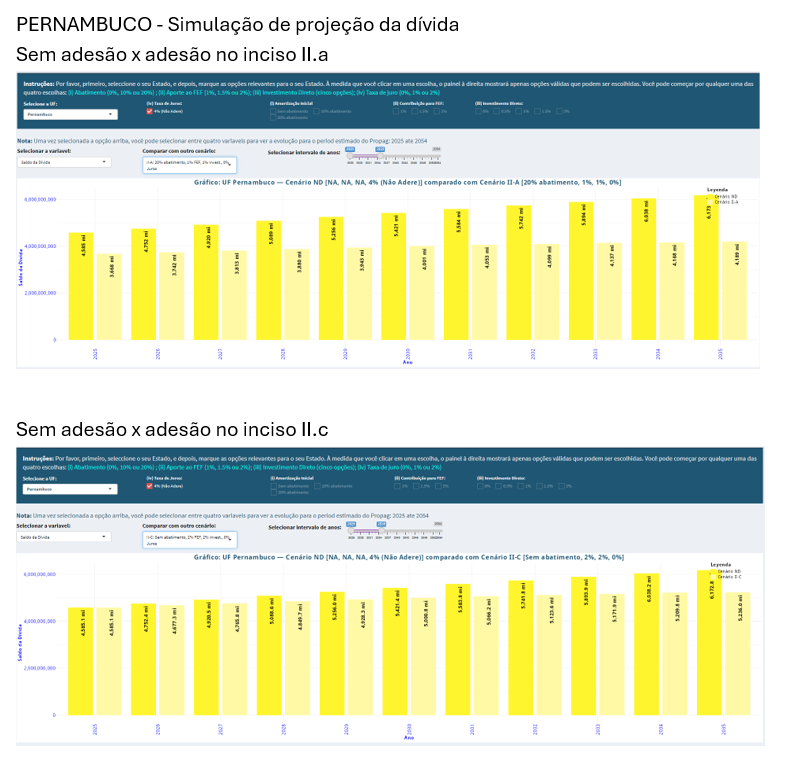
\includegraphics[width=1\textwidth]{images/7b.png}
	\caption{Aba E: Análise de Cenários EPT} 
	\label{fig:7b}
\end{figure}


\begin{figure}[htbp!]
	\centering
	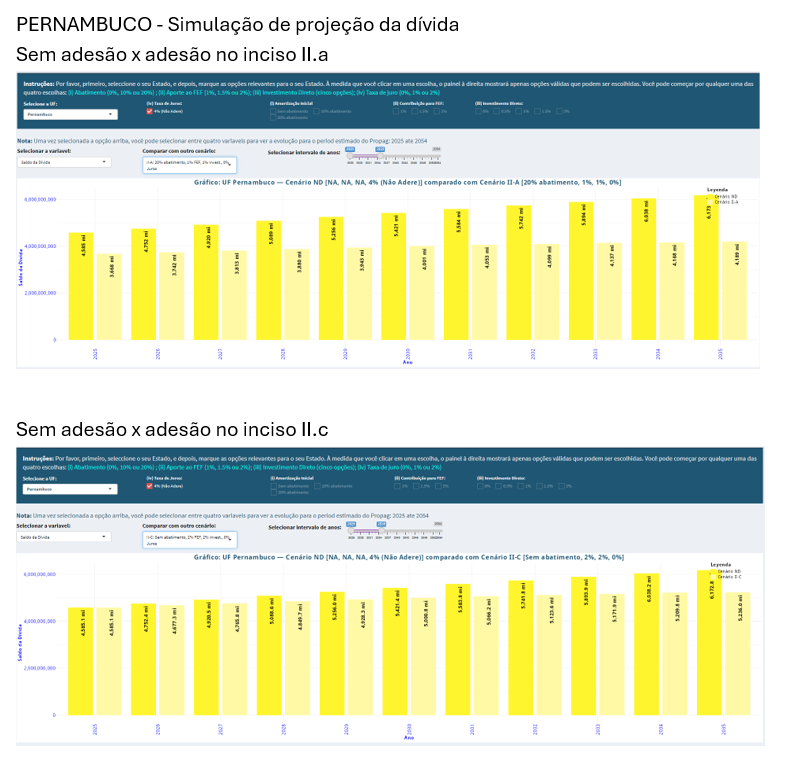
\includegraphics[width=1\textwidth]{images/7b.png}
	\caption{Aba E: Análise de Cenários EPT} 
	\label{fig:7c}
\end{figure}


\section{Opções de adesão}

Os estados que optarem por aderir ao Propag, deverão escolher uma dentre as 8 formas de adesão ao programa.

São 3 opções de taxa de juros que irão incidir sobre o saldo devedor que são de 0\% (zero) no inciso II, 1\% (um por cento) no inciso III e 2\% (dois por cento) no inciso IV. 

Além da escolha da taxa de juros, o estado deverá escolher uma das opções de amortização do saldo devedor, que pode ser de 0\% (zero), 10\% (dez por cento) ou 20\% (vinte por cento) que irão incidir sobre o valor do saldo devedor. Nesta amortização, o estado poderá oferecer ativos à União, como bens móveis e imóveis, créditos, participações societárias, etc., como forma de abatimento.

Cumpre lembrar que, mesmo os estados que não possuem dívidas com a União, poderão aderir ao Propag, e poderão participar da distribuição dos recursos do Fundo de Equalização Federativa, sem a necessidade de contribuir para este fundo.

Conforme a opção do estado, por taxa de juros e percentual de amortização, ele se enquadrará em uma das opções da tabela abaixo no que diz respeito ao percentual de aporte e de investimentos internos diretos:


\begin{figure}[htbp!]
	\centering
	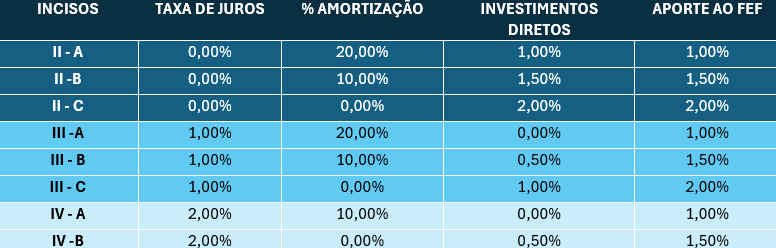
\includegraphics[width=1\textwidth]{images/7_opcoes.png}
	\caption{Aba E: Análise de Cenários EPT - Opções } 
	\label{fig:7_opcoes}
\end{figure}


\subsection{Simulação comparativa das opções de adesão}

Com o objetivo de realizar um comparativo entre duas das oito opções de adesão ao Propag, apresenta-se abaixo, algumas simulações de aporte ao FEF com os estados optando por aderir na opção do inciso II.a, com taxa de juros 0\% e 20\% de amortização do saldo devedor em comparação com a opção de adesão do mesmo estado no inciso II.c, com taxa de juros 0\% e amortização de 0\% sobre o saldo devedor.


\begin{figure}[htbp!]
	\centering
	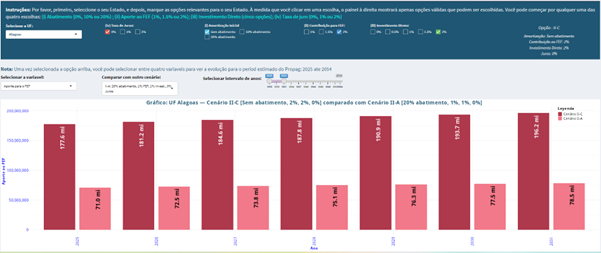
\includegraphics[width=1\textwidth]{images/7f.png}
	\caption{Simulação de Aporte ao FEF - Alagoas: Opção II.a x Opção II.c} 
	\label{fig:7f}
\end{figure}

\begin{figure}[htbp!]
	\centering
	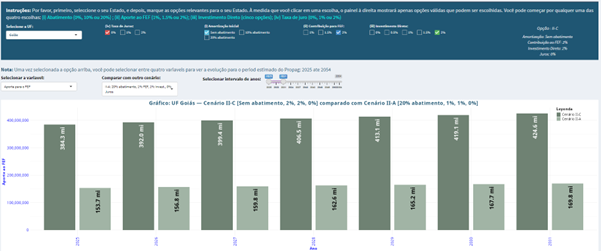
\includegraphics[width=1\textwidth]{images/7g.png}
	\caption{Simulação de Aporte ao FEF - Goiás: Opção II.a x Opção II.c} 
	\label{fig:7g}
\end{figure}

\begin{figure}[htbp!]
	\centering
	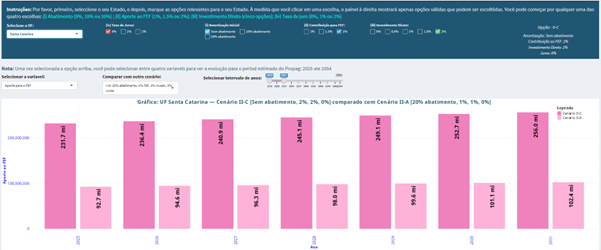
\includegraphics[width=1\textwidth]{images/7h.png}
	\caption{Simulação de Aporte ao FEF - [Estado]: Opção II.a x Opção II.c} 
	\label{fig:7h}
\end{figure}


\section{Simulação de retorno do FEF}

O Fundo de Equalização Federativa (FEF), é formado pelo aporte anual de percentual do saldo devedor dos estados que aderirem ao programa Propag, conforme as opções apresentadas anteriormente.

Após realizado o aporte pelos entes participantes, o valor resultante é dividido entre todos os estados que aderirem ao Propag, independentemente de ter ou não saldo devedor com a União.

O percentual de participação de cada estado é determinado pelo art. 46, incisos I e II do Decreto 12.433/2025, que estipula que a remuneração terá como critérios, o inverso da relação entre a Dívida Consolidada e a Receita Corrente Líquida com peso de 20\%, e o coeficiente de participação no Fundo de Participação dos Estados, com peso de 80\%.

A seguir, optou-se por representar um gráfico com uma simulação do valor devido para alguns estados, com 3 cenários diversos, conforme segue:

\begin{enumerate}
	\item Uma projeção simulada com a participação de todos os estados aderindo ao Propag pelo inciso II.a, com juros 0\% e amortização do saldo devedor de 20\%.
	\item Uma projeção simulada com a participação de todos os estados aderindo ao Propag, pelo inciso II.b, com juros 0\% e amortização do saldo devedor de 10\%.
	\item Uma projeção simulada com a participação de todos os estados aderindo ao Propag, pelo inciso II.c, com juros 0\% e amortização do saldo devedor de 0\%.
\end{enumerate}

\begin{figure}[htbp!]
	\centering
	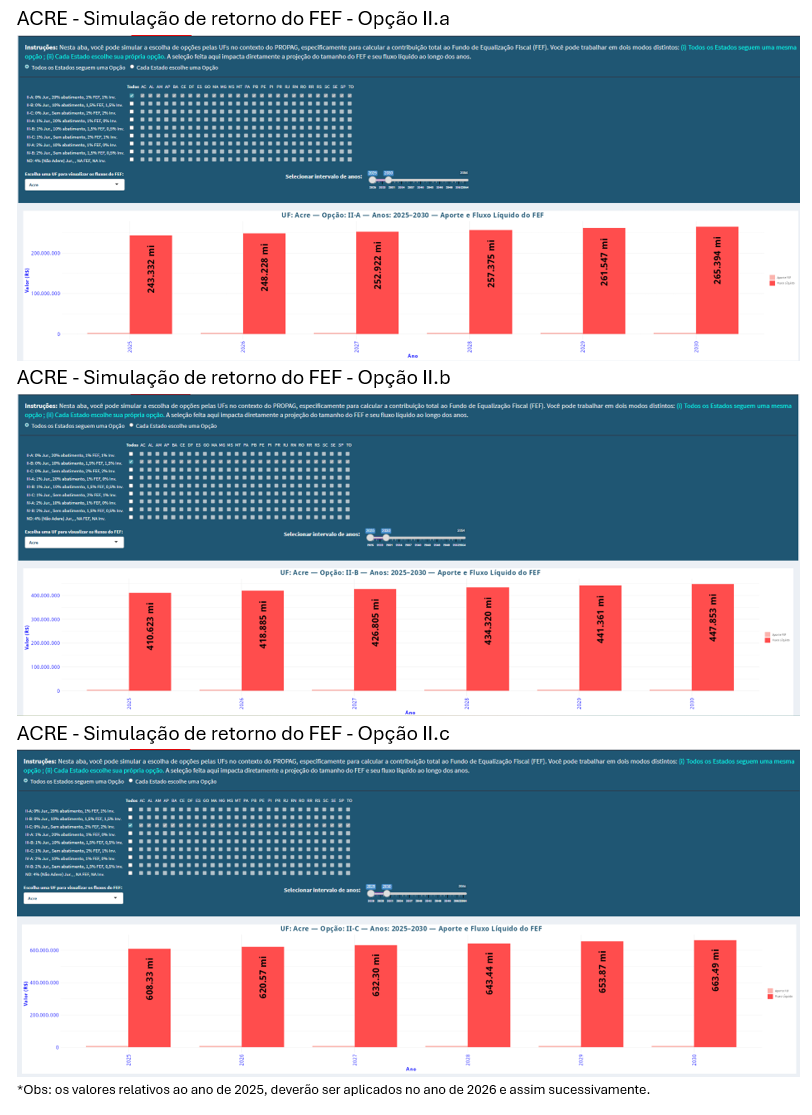
\includegraphics[width=1\textwidth]{images/7m.png}
	\caption{Simulação de Retorno do FEF - Acre: Comparação das Opções II.a, II.b e II.c} 
	\label{fig:7m}
\end{figure}


\begin{figure}[htbp!]
	\centering
	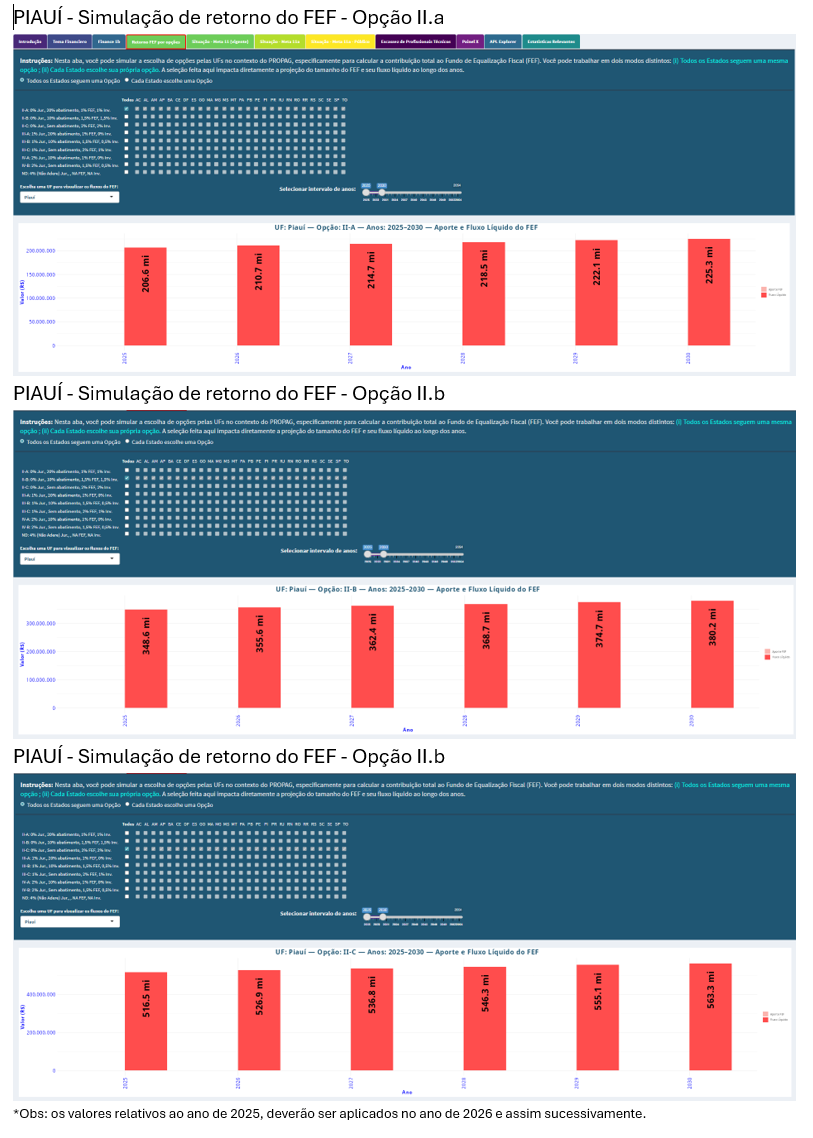
\includegraphics[width=1\textwidth]{images/7n.png}
	\caption{Simulação de Retorno do FEF - Piauí: Comparação das Opções II.a, II.b e II.c} 
	\label{fig:7n}
\end{figure}